% The results are subdivided in water demand, least-cost treatment systems, energy requirements, groundwater stress and sensitivity analysis, and are presented for an average year withing the 35 year analysis period.
\subsection{Water demand}
\begin{figure*}[!b]
	\centering
	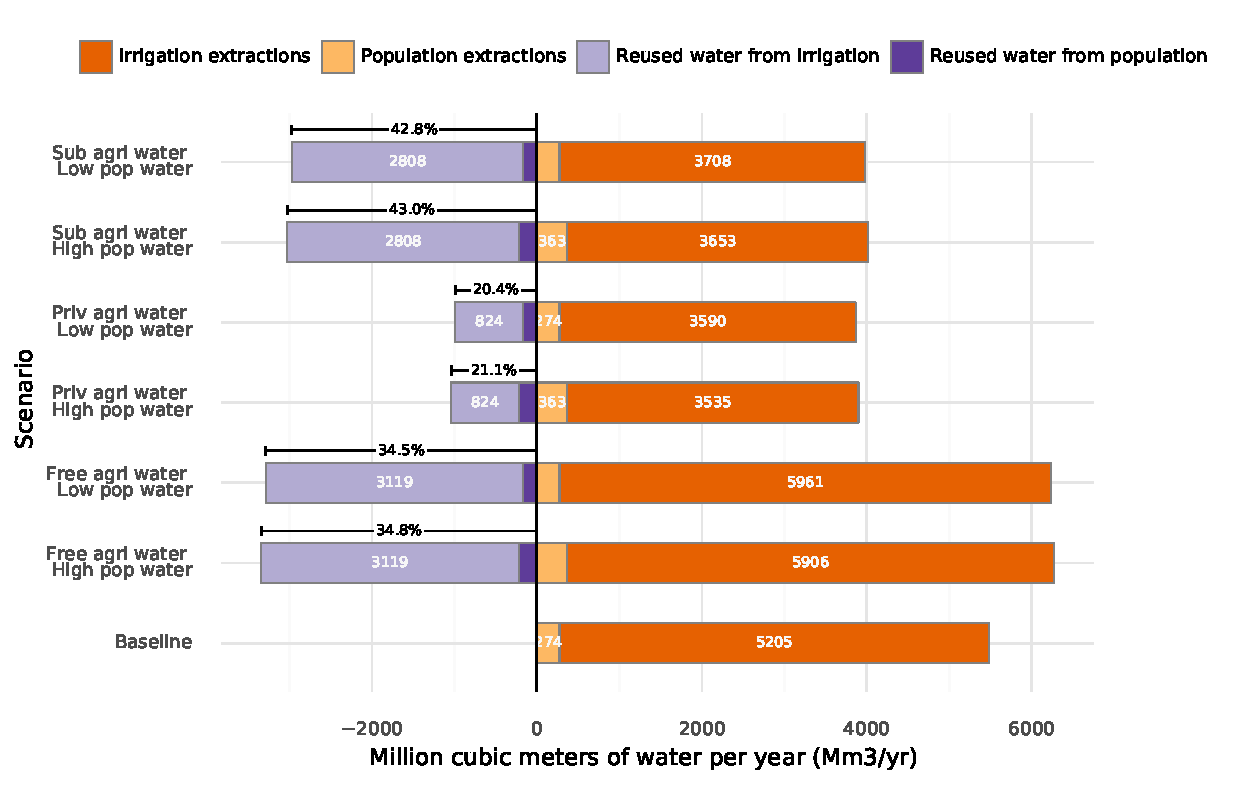
\includegraphics[width=0.8\textwidth]{Water}
	\caption{Water usage for all scenarios. At left: reused water after reclaim, treatment and allocation classified by population and irrigation source. Percentage bars indicate the share of reused water against the total demand. At right: overall water extractions classified by population and irrigation use. Percentage bars indicate the percentage of water saved compared to Baseline withdrawals}
	\label{fig:water}
\end{figure*}
Year average water withdrawals in the Baseline scenario were estimated at 4,141 Mm\textsuperscript{3}/yr, with agricultural irrigation accounting for 93\% of the total share (see \fref{fig:water} and \tref{tbl:resultswater}). In scenarios 1 and 2, the overall water used was lower than the Baseline scenario (i.e water withdrawals plus water reused), opposite behaviour to scenarios 3 and 4. However, due to the reused treated wastewater/tailwater in irrigation, the overall water withdrawals were lower than those of the Baseline. This shows that even in the worst case scenario of water usage (i.e. scenario 4), the total withdrawals can be reduced by treating and reusing wastewater/tailwater. Moreover, water withdrawals in scenarios 1 and 2 were very close to each other and lower than that of scenario 3. This suggests that the higher irrigation water price due to the private regime, promotes the use of more efficient irrigation schemes reducing even more water withdrawals compared to wastewater/tailwater reuse only.

\begin{table}[!ht]
	\caption{\label{tbl:resultswater}Summary of water results by scenario. The total for the entire aquifer (total), as well as the minimum (min), maximum (max), average (mean) and median values between the clusters are presented.}
	\footnotesize
	\lineup
	\begin{tabular*}{\textwidth}{@{}*{7}{l}}
		\br
		&        & \centre{5}{Scenario} \\
		\ns
		&        & \crule{5} \\
		Parameter & Value  &  Baseline &  Scenario 1 &  Scenario 2 &  Scenario 3 &  Scenario 4 \\
		\mr
		Water withdrawals (MCM) & total &    4141.7 &      2342.6 &      2244.6 &      2388.4 &      3958.1 \\
		& min &       0.6 &         0.6 &         0.6 &         0.6 &         0.6 \\
		& max &     502.6 &       284.2 &       284.2 &       284.9 &       494.3 \\
		& mean &     103.5 &        58.6 &        56.1 &        59.7 &        99.0 \\
		& median &      49.1 &        23.6 &        23.6 &        25.5 &        44.7 \\
		Water reused (MCM) & total &    0 &      1669.3 &      1022.1 &      2264.0 &      2385.0 \\
		& min &       0.0 &         0.0 &         0.0 &         0.0 &         0.0 \\
		& max &     0 &       212.4 &       119.1 &       296.5 &       304.4 \\
		& mean &      0 &        41.7 &        25.6 &        56.6 &        59.6 \\
		& median &      0 &        15.7 &        13.2 &        28.1 &        29.3 \\
		Water savings (MCM) & total &       0.0 &      1799.1 &      1897.2 &      1753.4 &       183.7 \\
		& min &       0.0 &         0.0 &         0.0 &         0.0 &       -27.1 \\
		& max &       0.0 &       218.5 &       225.0 &       217.7 &        66.7 \\
		& mean &       0.0 &        45.0 &        47.4 &        43.8 &         4.6 \\
		& median &       0.0 &        19.0 &        19.5 &        17.1 &         2.9 \\
		\br
	\end{tabular*}
\end{table}

The share of reused wastewater/tailwater in the total water used was highest in scenario 3 (48.7\%) and lowest in scenario 2 (31.3\%). This means, that the available tailwater to reclaim, treat and reuse is much lower in scenario 2. As the overall irrigation efficiency is better in Scenario 2, the available tailwater to reclaim is lower, thus the reused share in the total water used is reduced. However, this is compensated with the reduced water withdrawals due to lower water use. This shows again the importance of using efficient irrigation schemes in reducing total water withdrawals.

On the other hand, wastewater/tailwater reuse share was lower in scenario 4 against scenario 3. This was due to the cap set to the on-farm storage area of maximum 2\% share of the cropland area. Therefore, while more recoverable water is available in scenario 4 (i.e. due to the free water regime), the storage system cannot hold everything.
% This could be solved by setting a higher value for the permissible on-farm storage area, however, this would mean that more agricultural area would be used for storage purposes, possibly having trade-offs with target 2.3 of SDG 2 on doubling agricultural productivity and incomes of small-scale food producers.

Domestic water withdrawals do not represent large shares in the overall water use, as irrigation water use are much more extensive. Nonetheless, with the use of more efficient irrigation schemes and population growth, recoverable irrigation tailwater decreases, and population treated wastewater share on agricultural water usage increases. Detailed per cluster results are presented in section 10 of the \textit{supplementary information}.

\subsection{Least-cost wastewater treatment systems}
Intermittent sand filters, rotating biological contractors and extended aeration were the least-cost technologies identified for domestic wastewater treatment, with 1.8\%, 11.7\% and 86.4\% share respectively. \Fref{fig:lcowbaseline}, shows the LCOW value comparison of the technologies in evaluation, against the required treatment capacity of each cluster. In general, when lower capacity is required simpler treatment technologies are more cost-effective, as the independent variable of the CAPEX and OPEX cost functions is the available reclaimed wastewater flow.

\begin{figure*}[!h]
	\centering
	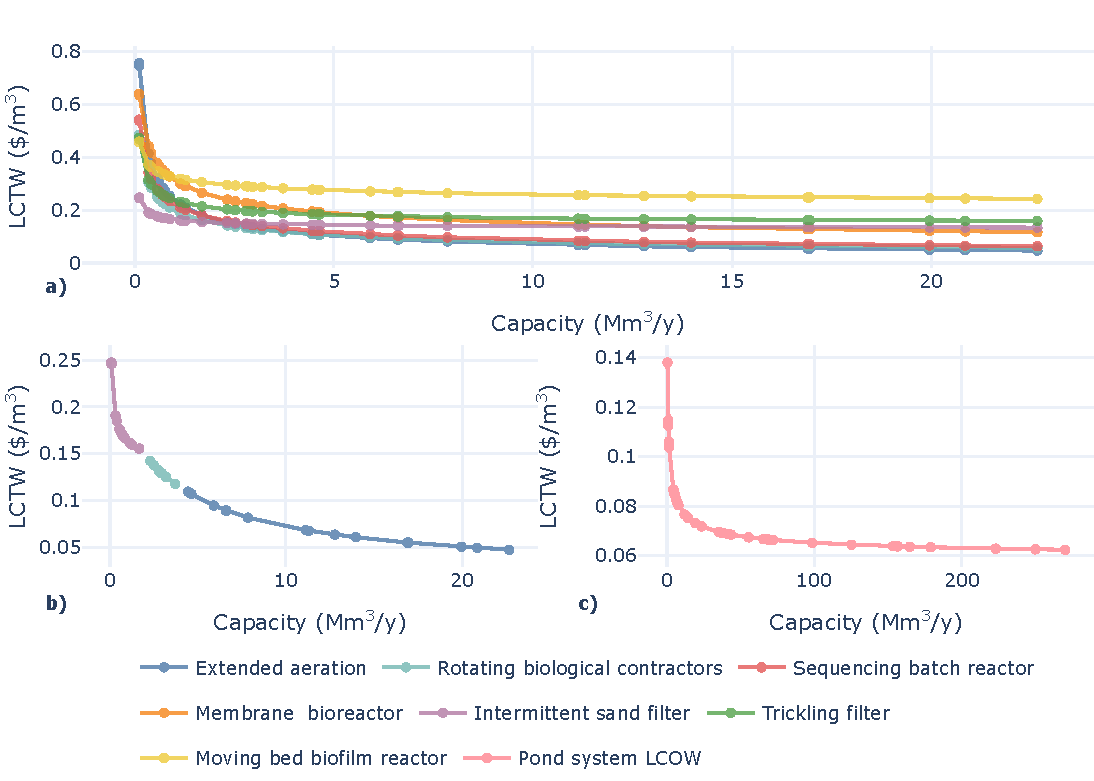
\includegraphics[width=0.9\textwidth]{lcowPopAg}
	\caption{Levelized cost of water (LCOW) against treatment capacity for each cluster in Scenario 1. \textbf{a)} LCOW for the 7 different technologies evaluated for domestic wastewater treatment. \textbf{b)} Least-cost technologies for population wastewater treatment. \textbf{c)} LCOW of the pond systems treatment technology evaluated for irrigation tailwater.}
	\label{fig:lcowbaseline}
\end{figure*}

% \begin{figure*}[!ht]
% 	\centering
% 	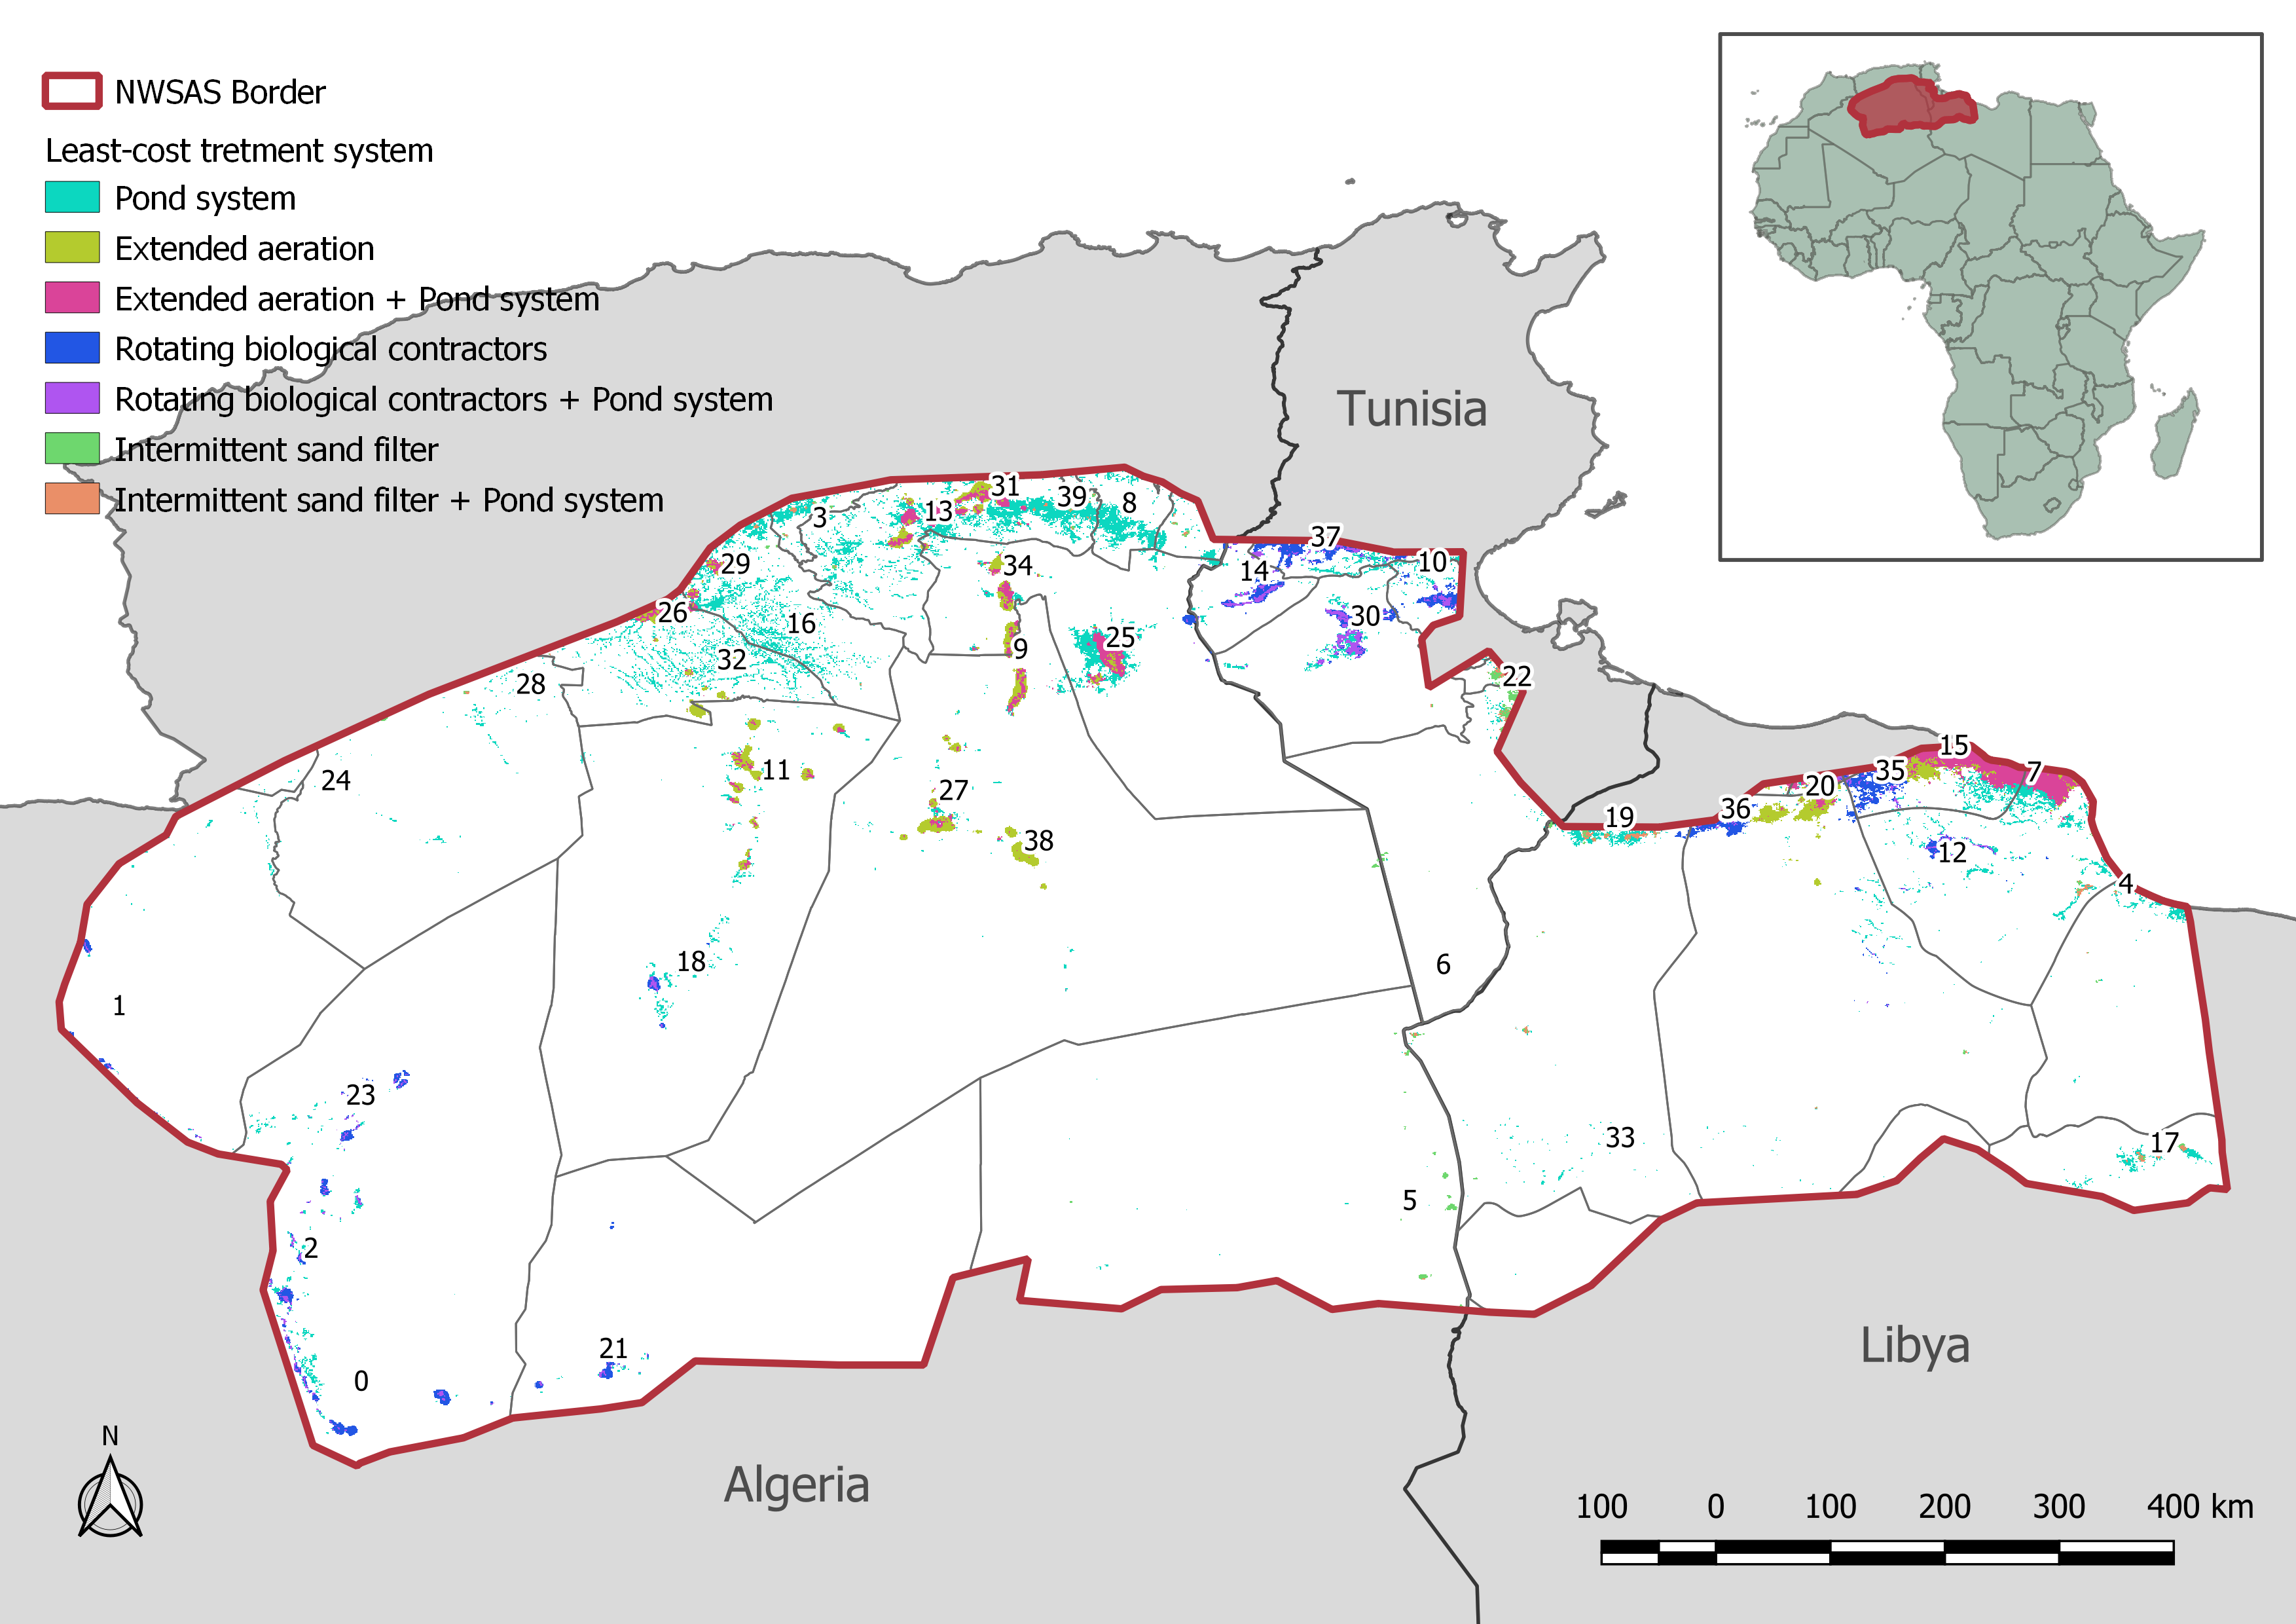
\includegraphics[width=0.88\textwidth, cfbox=black 1pt 0pt]{NWSAS_least-cost_system_cluster}
% 	\caption{Least-cost wastewater treatment options per cluster---low population water requirements.}
% 	\label{fig:leastLow}
% \end{figure*}

% \begin{figure*}[!ht]
% 	\centering
% 	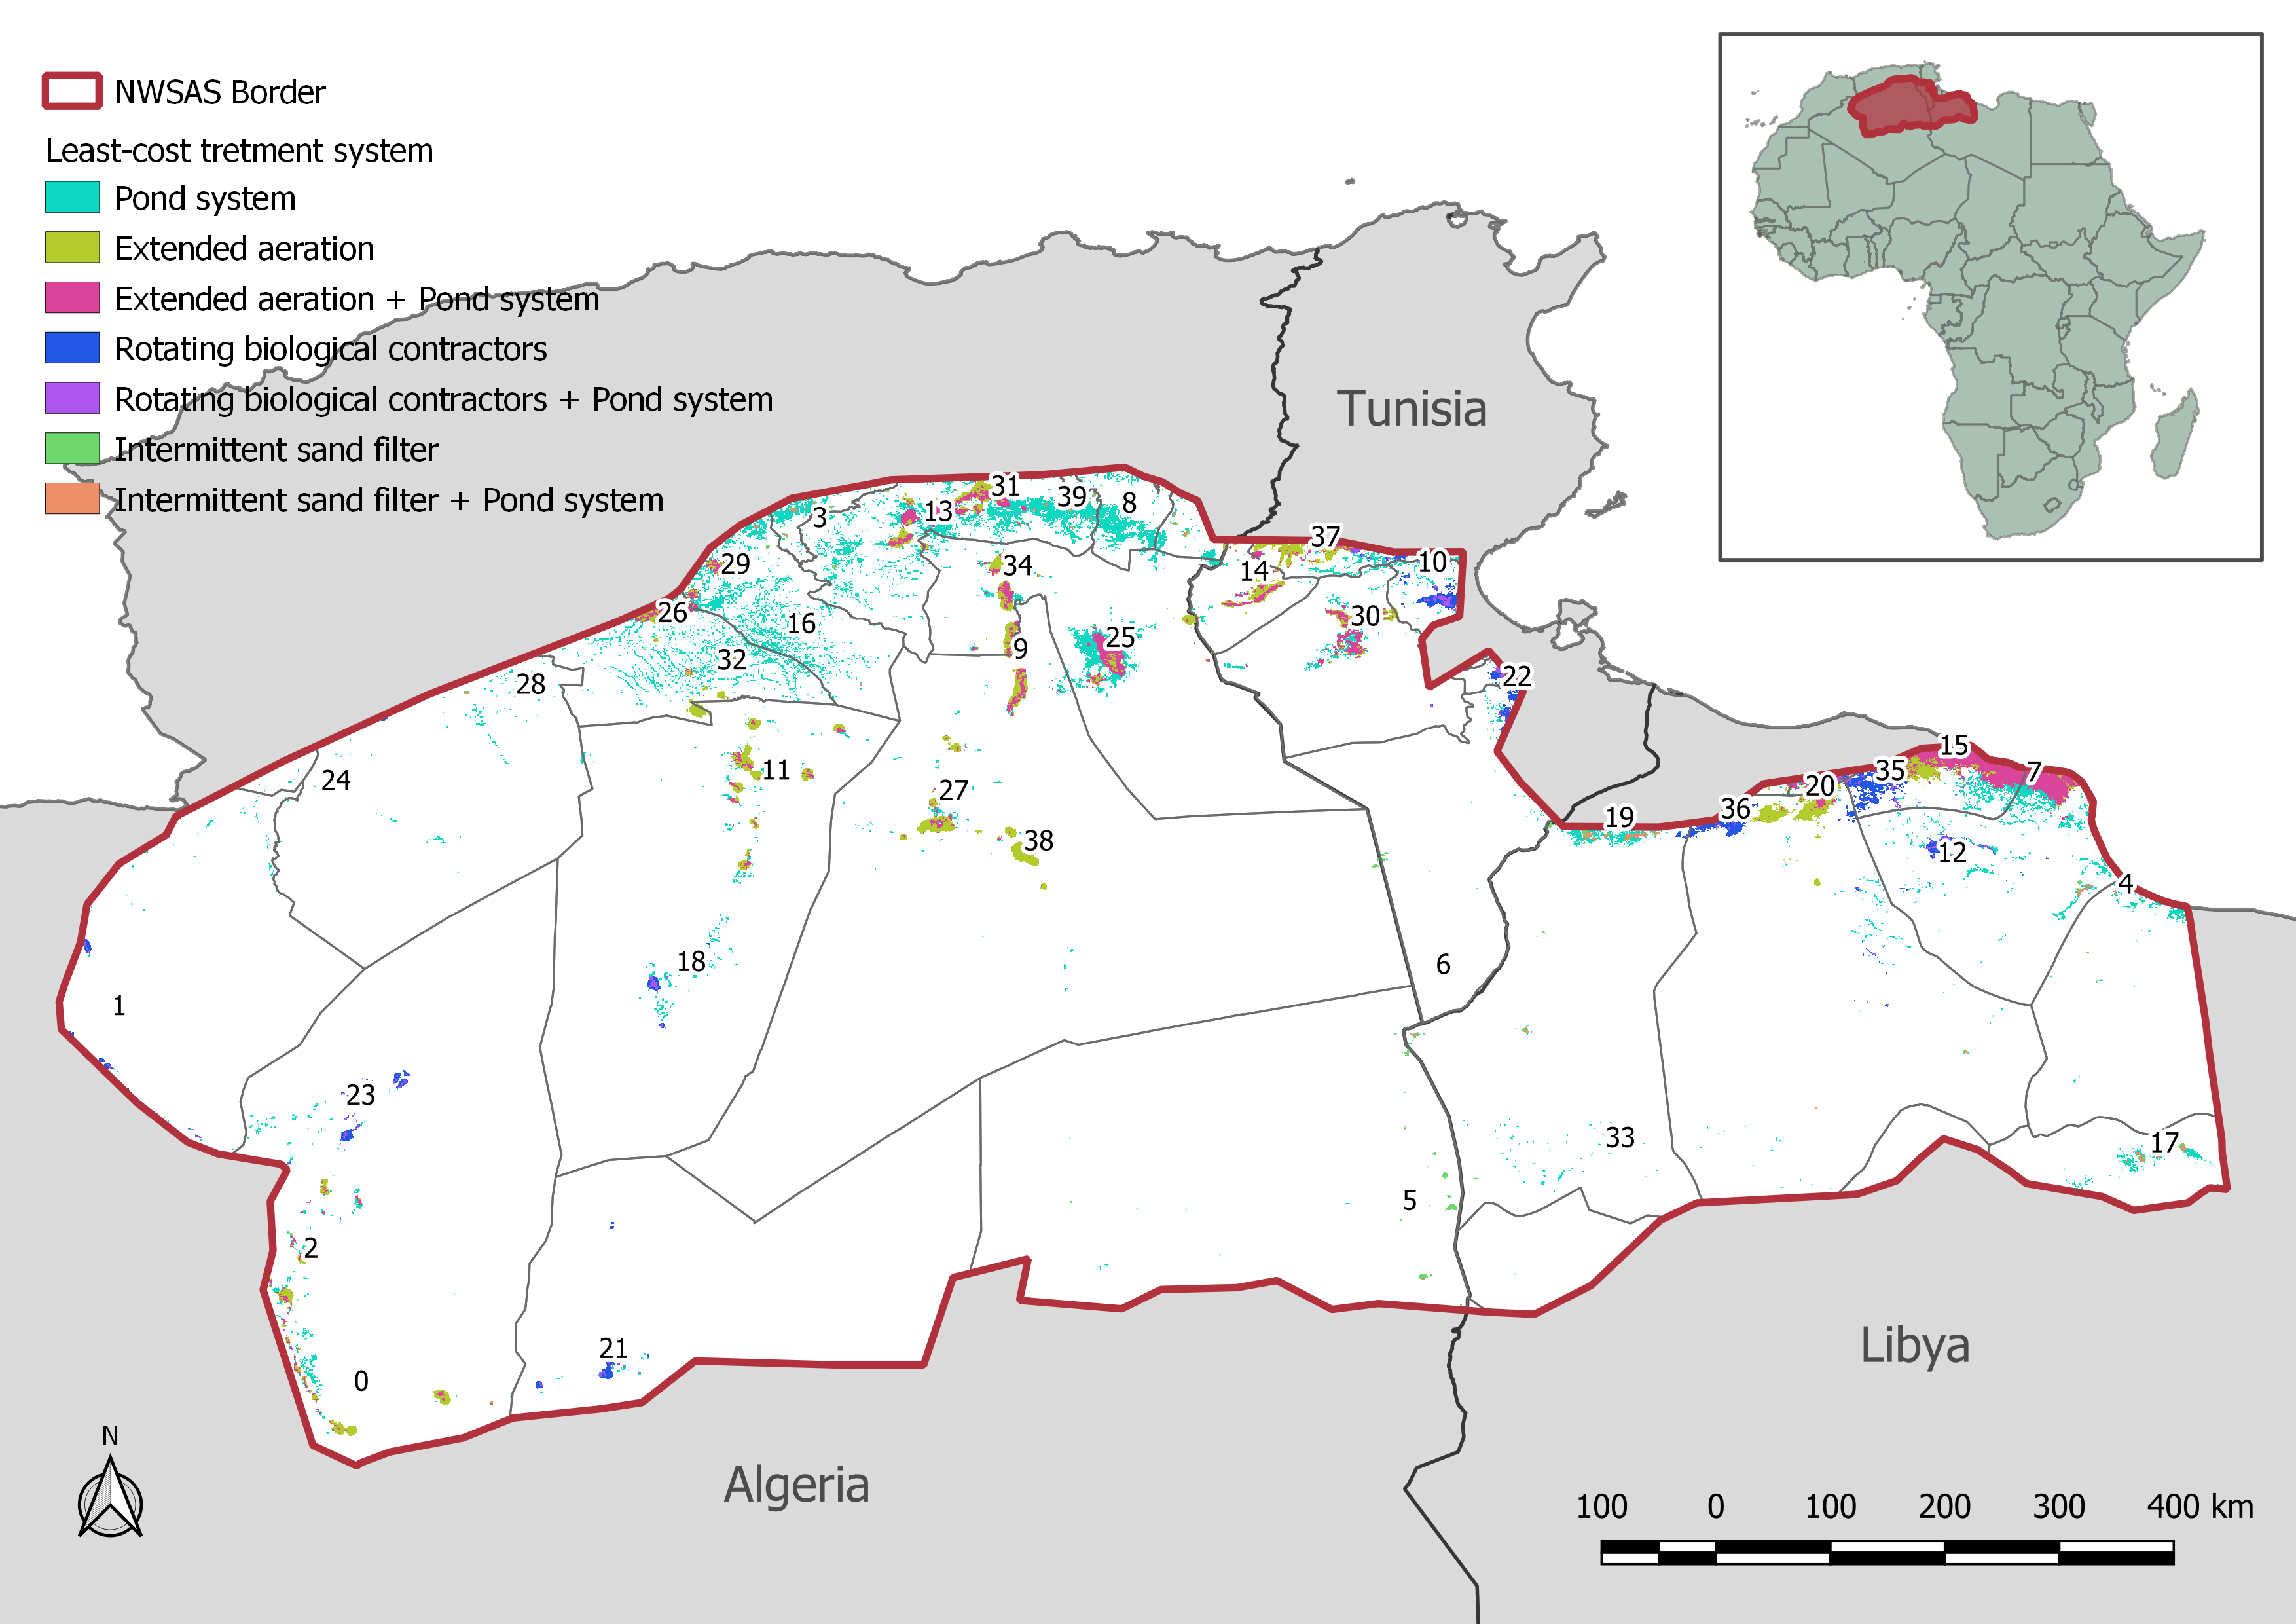
\includegraphics[width=0.88\textwidth, cfbox=black 1pt 0pt]{NWSAS_least-cost_system_cluster_high}
% 	\caption{Least-cost wastewater treatment options per cluster---high population water requirements.}
% 	\label{fig:leastHigh}
% \end{figure*}

The previous is important, as the amount of wastewater available from the agglomerations is key for the calculation of the least-cost technology. Therefore, with larger agglomerations, scalable and higher capacity systems could be implemented. 
% The downside however, is that if the costs related to the conveyance system are not evaluated, then the distances among population and/or irrigation points become irrelevant, which is arguably far from reality. Thus, the analysis of more compact clusters, reduces the drawbacks of not calculating the costs related to a wastewater conveyance system.

Moreover, the LCOW value for tailwater treatment in pond systems, shows a steep increase in value for very low treatment capacity. This implies that as irrigation efficiency or irrigated area decreases, the cost feasibility of using pond systems also decreases.

Overall, the least-cost treatment systems obtained, showed important trade-offs, as the best solutions are dependent on geospatial factors than can render a specific technology less costly than other in a given region. Parameters as population proximity to irrigated areas, wastewater treatment capacity and irrigation water usage are key for selecting the proper wastewater treatment and reuse systems. Detailed cluster maps on least-cost technologies can be found in section 12 of the \textit{supplementary information} and sensitivity analysis on discount rate on section 13.

\subsection{Energy requirements}
\begin{figure*}[!b]
\centering
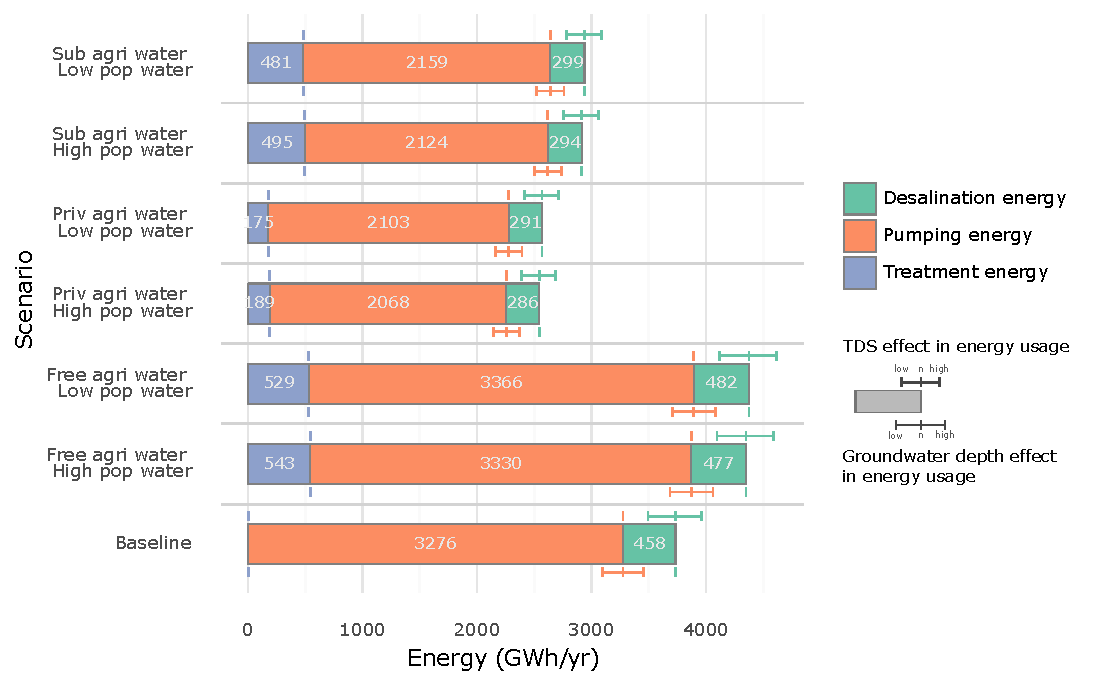
\includegraphics[width=0.9\textwidth]{Energy}
\caption{Energy requirements for all scenarios. Percentage bars indicate the share of saved energy against the baseline total.}
\label{fig:energy}
\end{figure*}

The overall energy related outcomes for all scenarios are shown in \fref{fig:energy} and \tref{tbl:resultsenergy}. The energy requirements for groundwater pumping represent the major part of all three activities. Desalination energy, although smaller, represent about one third as much as pumping energy. All scenarios apart from Scenario 4, reduced overall energy consumption compared to the Baseline. 

\begin{table}[!ht]
	\caption{\label{tbl:resultsenergy}Summary of energy results by scenario. The total for the entire aquifer (total), as well as the minimum (min), maximum (max), average (mean) and median values between the clusters are presented.}
	\footnotesize
	\lineup
	\begin{tabular*}{\textwidth}{@{}*{7}{l}}
		\br
		&        & \centre{5}{Scenario} \\
		\ns
		&        & \crule{5} \\
		Parameter & Value  &  Baseline &  Scenario 1 &  Scenario 2 &  Scenario 3 &  Scenario 4 \\
		\mr
		Energy (GWh) & total &    3055.7 &      2866.8 &      2688.7 &      2951.1 &      4721.5 \\
         & min &       0.5 &         0.8 &         0.8 &         0.8 &         0.8 \\
         & max &     402.8 &       375.0 &       360.6 &       388.9 &       641.8 \\
         & mean &      76.4 &        71.7 &        67.2 &        73.8 &       118.0 \\
         & median &      26.7 &        27.7 &        26.6 &        28.8 &        48.1 \\
		\br
	\end{tabular*}
\end{table}

Such reductions, are achieved by the reuse of treated wastewater in irrigation, as the energy intensity of treatment is substantially lower than the energy intensity for pumping water from the deep aquifer. This shows synergies between SDG 6, SDG 2 and SDG 7, as when more wastewater is collected and treated it can be made available for reuse in agriculture, supporting sustainable food production and efficient irrigation schemes. Moreover, it can reduce energy intensity of the system and promote the use of clean energy sources. Additional results are presented in section 11 of the \textit{supplementary information}.

\begin{figure*}[!b]
	\centering
	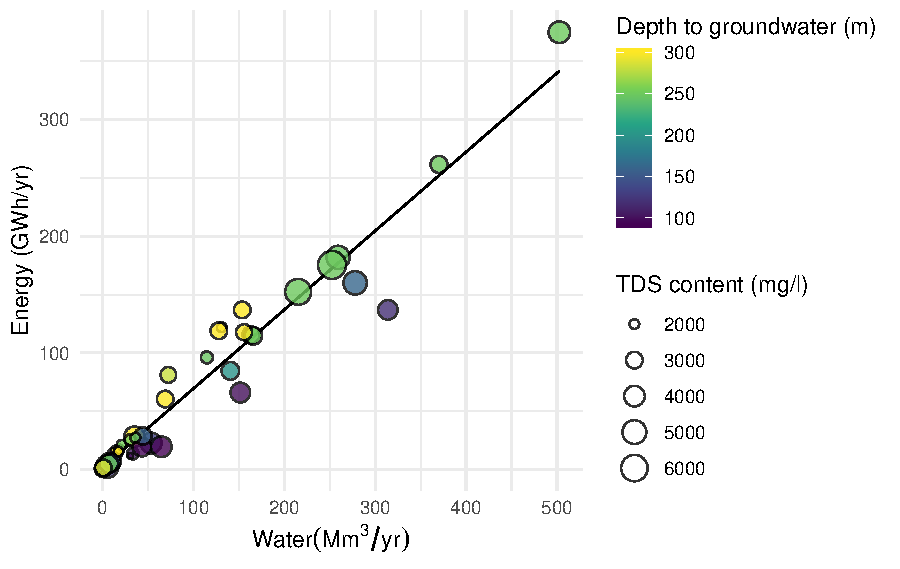
\includegraphics[width=0.7\textwidth]{Images/NexusPlotWithReuse.pdf}
	\caption{Total energy and water requirements per cluster for Scenario 1. Clusters are represented by the data points. TDS contents of water (mg/l) are shown as the size parameter of each data point/cluster. Depth to groundwater (m) is represented by the color ramp. The diagonal represents the trend line of the data points.}
	\label{fig:energyclusters}
\end{figure*}

 Moreover, TDS content of brackish water is important in defining the desalination energy requirements, however as identified in \cite{karabelasAnalysisSpecificEnergy2018a,panBrackishWaterDesalination2020}, the main driver for energy needs in RO desalination is for the feed water pressurization. This can be seen in \fref{fig:energyclusters} where all clusters having lower depth values are consistently placed to the right side of the diagonal. The opposite is true for clusters with higher depth levels. On the other hand, TDS content seems to have a much weaker effect. Details of the methodology used for estimating desalination energy requirements can be seen section 7 of the \textit{supplementary information}  and section 13 presents sensitivity analysis on TDS content of brackish water. 

% Key parameters to define total energy requirements for pumping and desalination are depth to groundwater and TDS content of the water (see \fref{fig:energyclusters}). The depth to groundwater has a stronger impact on the overall energy requirements, as can be evidenced in \fref{fig:energyclusters}, where all clusters having lower depth values are consistently placed to the right side of the diagonal. The opposite is true for clusters with higher depth levels. On the other hand, TDS content seems to have a much weaker effect. This suggests that, increasing water table levels is a crucial parameter to take into account for energy supply planning. It can significantly affect pumping energy requirements, but as well reduce the water productivity of the region. Nonetheless, reduced quality levels of water (i.e. higher TDS content) could have severe consequences on health and crop productivity (variables that were not accounted for in this study).

\subsection{Groundwater Stress}
The overall aquifer GWS for all scenarios, falls inside the extremely high category (\tref{tbl:gws} and \fref{fig:gws}). Moreover, the indicator distribution throughout the clusters vary widely, with some clusters falling inside the low and low-to-medium categories. This behaviour is mainly driven by the differences in irrigated area withing each cluster and the cluster area. Nonetheless, all scenarios achieved a reduction in GWS due to the reduction on total water withdrawals. Scenario 3, 1 and 2 achieved substantial reductions of around 42\%, 43\% and 46\% respectively. Total, min, max, mean, and median values of GWS are presented in \tref{tbl:gws}.

\begin{table}[!h]
	\caption{\label{tbl:gws}Summary of GWS results by scenario. The total for the entire aquifer (total), as well as the minimum (min), maximum (max), average (mean) and median values between the clusters are presented.}
	\lineup
	\footnotesize
	\begin{tabular}{@{}*{7}{l}}
		\br
		&        & \centre{5}{Scenario} \\
		\ns
		&        & \crule{5} \\
		Parameter & Value  &  Baseline &  Scenario 1 &  Scenario 2 &  Scenario 3 &  Scenario 4 \\
		\mr
GWS (-) & total &     121.0 &        68.5 &        65.6 &        69.8 &       115.7 \\
        & min &       5.9 &         3.2 &         3.2 &         3.2 &         4.2 \\
        & max &     461.8 &       260.9 &       260.9 &       260.9 &       432.3 \\
        & mean &     135.5 &        81.4 &        79.2 &        82.3 &       130.8 \\
        & median &      89.5 &        58.5 &        58.5 &        63.5 &        94.8 \\
Water stress (\%) & total &     375.7 &       212.5 &       203.6 &       216.7 &       359.0 \\
        & min &      18.2 &        10.0 &         9.9 &         9.9 &        12.9 \\
        & max &    1433.6 &       809.9 &       809.9 &       809.9 &      1341.9 \\
        & mean &     420.5 &       252.6 &       245.8 &       255.4 &       406.2 \\
        & median &     277.7 &       181.5 &       181.5 &       197.1 &       294.1 \\
		\br
	\end{tabular}
\end{table}

The GWS can be related to SDG target 6.4.2 on Water Stress, which measures the share of total water withdrawals over the total renewable water resources, subtracting environmental flow requirements. Both indicators are broadly consistent and clearly show the critical condition of the region in terms of water scarcity (see \tref{tbl:gws}). Synergies and trade-offs of SDG 2 with SDG 6 are clear, specially with targets 6.4 on increasing water-use efficiency and ensuring sustainable withdrawals and supply of freshwater to ease water scarcity, and 6.6 on protect and restore water-related ecosystems.

\begin{figure}[!t]
	\centering
	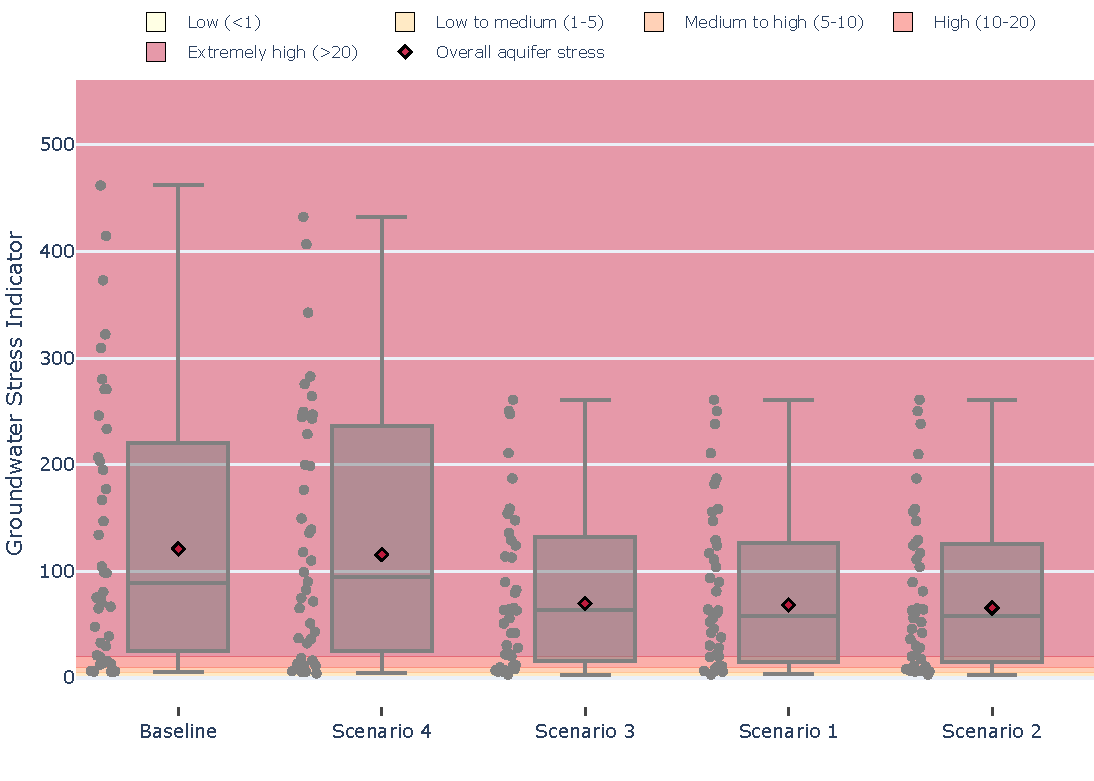
\includegraphics[width=0.9\textwidth]{GWS}
	\caption{Groundwater stress indicator for all scenarios. The distribution of the indicator throughout the 40 clusters is represented by the points and the boxes, whereas the overall indicator calculated for the entire basin is represented by the red diamonds. The background indicates the scale of stress that the indicator falls into.}
	\label{fig:gws}
\end{figure}

% \subsection{Sensitivity analysis}
% The sensitivity analysis demonstrates how a change of \rpm10 meters in the depth to groundwater level, has an average variation of circa \rpm5.5\% over the overall pumping energy requirements. Moreover, desalination energy requirements showed variations of $-$53\% to $+$50\%, when changes of \rpm50\% in the TDS levels were considered.

% These effects on the energy-for-water requirements, are necessary to be assessed when planning for new water policies and water management strategies. Accordingly, accounting for new energy infrastructure, or potential energy savings could be key for the success of a new policy or solution to the water scarcity problem.